% !Mode:: "TeX:UTF-8"
% !TEX root = ..\Literature_Translation.tex
\stepcounter{app}
\setcounter{figure}{0}
\setcounter{table}{0}
\newpage
\begin{Abstract}
\chapter*{航空工厂的装配夹具生产调度}\addcontentsline{toc}{section}{航空工厂的装配夹具生产调度}
\begin{center}
\vspace{2mm}
{
 {\xiaosi Bruno Jensen Virginio da Silva$^a$,  Reinaldo Morabito$^a$, Denise Sato Yamashita$^a$,\\ Horacio Hideki Yanasse$^b$}

 {\xiaowu $^a$Departamento de Engenharia de Produção, Universidade Federal de São Carlos, Brazil\\
 $^b$Nati Instituto de Ciência e Tecnologia, Universidade Federal de São Paulo, Brazil}
}
\end{center}
{\songti
\noindent \xiaowu\textbf{摘要:}我们将在本文研究在航空工厂的装配生产调度问题。飞机零件需要在夹具上生产制造,这在飞机制造上是很常见的,而且会由多个
工作站组成。由于夹具的物理工件小,当一个工作站在工作的时候,与其相邻的工作站便无法工作,这些约束称为邻接约束。该装配夹具调度问题的研究背景是,将员工的学习进程分为4个主要限制阶段(或时期)。最优化求解器和建模语言将运用到各阶段的数学建模和应用。该方法的计算实验将被运行在一个巴西航空工厂的案例研究,并可以得到该方法比现行方法要好的结论。

\keywords{生产调度、装配夹具、航空工厂、邻接约束}
}
\end{Abstract}
% !Mode:: "TeX:UTF-8"
% !TEX root = ..\Literature_Translation.tex
\kchapter{引言}
我们将在本文描述一个产生于飞机制造的装配夹具的生产调度问题。
我们对受邻接约束下,为了装配而用到夹具的这部分特殊飞机零件的生产特别感兴趣。夹具是用来夹紧工件或作为支撑的设备,专为适用特定零件或形状而建。
夹具的主要作用是定位,在某些情况下也用于整个加工操作中或其他工业过程的工件保持(Niu,1988;Drake,1989;Howe,2004)。
由于空间限制,夹具相邻的工作站不能同时开工,产生了邻接约束。
装配一个飞机零件至少需要2个步骤,其中之一需要在夹具上完成,另一个互补的装配操作将在工作台上进行。根据装配所需的零件,这两个操作需要重复操作。


% !Mode:: "TeX:UTF-8"
% !TEX root = ..\Literature_Translation.tex
\kchapter{阶段建模}
\ksection{阶段1}
阶段1的目标是找到只有1个装配夹具,而不顾可用工人数时的最大生产能力,即工人数量无限的情况下最小化制造期。
接下来的模型是基于Coffman(1976), Baker(1974), Morton和 Pentico(1993), Leung(2004)和 Pinedo(2008), Potts和 Strusevich(2009)的作业车间调度问题。设$L$为任务数,对于每个任务$j=1,2,...,J$:\\[3pt]
\indent$p_j:$ 任务$j$在装配夹具的操作持续时间\\
\indent$q_j:$ 任务$j$在工作台的操作持续时间

此外,需要对每个任务对$(j,k),j\neq k$定义集合如下:
\begin{numcases}{}
A = \left\{(j,k)\mid\text{任务$j$需在任务$k$开始前结束}\right\}\notag\\
B = \left\{(j,k)\mid\text{任务$j$和任务$k$在夹具内的邻接工作台操作}\right\}\notag\\
C = \left\{(j,k)\mid\text{任务$j$和任务$k$在夹具内同一个位置操作}\right\}\notag
\end{numcases}

决策变量建模如下:
\vspace{-3pt}
\begin{numcases}{y_{jk} = }
1\qquad\text{如果任务$j$在任务$k$前调度}\notag\\
0\qquad\text{其他情况}\notag 
\end{numcases}

$t_j:$ 任务$j$的开始时间

$t_F:$ 制造期

那么阶段1的数学模型如下:
\begin{align}
&\label{equb:1} \min \quad t_f \\
&\label{equb:2} t_j + p_j + q_j \leqslant t_F \qquad j = 1,...,J\\
&\label{equb:3} t_k + M(1 - y_{jk}) \geqslant t_j + p_j \qquad \text{对于所有} (j,k)\in C\\
&\label{equb:4} t_j + M\times y_{jk} \geqslant t_k + p_k \qquad \text{对于所有} (j,k)\in C\\
&\label{equb:5} t_k \geqslant t_j + p_j + q_j  \qquad \text{对于所有} (j,k)\in A\\
&\label{equb:6} t_k + M(1 - y_{jk}) \geqslant t_j + p_j \qquad \text{对于所有} (j,k)\in B\\
&\label{equb:7} t_j + M\times y_{jk} \geqslant t_k + p_k \qquad \text{对于所有} (j,k)\in B\\
&\label{equb:8} t_j \geqslant 0,\ y_{jk}\in \{0,1\},\quad j=1,...,J,\quad k=1,...,J,\quad j\neq k
\end{align}

在模型(\ref{equb:1}) -- (\ref{equb:8})中,目标函数\eqref{equb:1}最小化了制造期$t_F$,约束\eqref{equb:2}保证了制造期要不小于任何调度内任务的完成时间。
约束\eqref{equb:3}和(\ref{equb:4})避免了在同个装配工作站的任务重叠,需要注意的是,这两约束只为同工作站装配任务对$j$和$k$定义。
也需注意的是约束\eqref{equb:3}和(\ref{equb:4})是相互分离的,即一个激活时,另一个是冗余的,反之亦然(William,1999)。
参数M 是一个足够大的正数,可以定义为:$\sum_{j=1}^J(p_j + q_j)$。
约束\eqref{equb:5}保证先后之间的关系。
约束\eqref{equb:6}和(\ref{equb:7})保证需要用到邻接工作站的任务不会同时被调度。
约束\eqref{equb:8}参考决策变量的定义域。

以防万一,包括一些任务可能在0时刻之后提交,并且有些任务可能有工期(即防止任务与多于1架飞机有关而产生不同的工期),我们可以定义:\\[3pt]
\indent $r_j:$ 任务$j$的提交日期

$d_j:$ 任务$j$的工期\\
这样一来上述模型可以简单地改变以包含下述约束:
\begin{align}
&\label{equb:9} t_j \geqslant r_j \qquad \text{对于一些$j$}\\
&\label{equb:10} t_j + p_j + q_j \leqslant d_j \qquad \text{对于一些$j$}
\end{align}
其中,\eqref{equb:9}保证每一个任务$j$都在其提交日期$r_j$之后才被调度,\eqref{equb:10}保证每个任务$j$都在工期$d_j$前完成。
同时注意参数M 需要相应修改以使提交日期$r_j$非空。

\ksection{阶段2}
在本阶段,要考虑2个装配队伍:夹具装配队伍和工作台队伍。
该阶段的目标是最小化总成本或人工数量,并且在给定工期前完成。
在一些变化后,该问题可以建模成考虑时间因素的项目调度问题。
这个项目包含多个活动,每个活动都需要1种以上的资源使其得以执行。
通常,活动有其已知的持续时间,并且由于技术限制,它们中间往往存在先后关系。
本文研究的项目调度问题考虑有限但可再生资源,即被使用过后,该资源可以再次被使用(员工、机器设备等都是可再生资源的例子)。
其目标是在最小化资源使用量,考虑活动的先后关系,可用资源量,以及在给定工期的前提下,找到一个可行调度。
在项目调度的范畴中,该问题以时间约束的项目调度闻名(Brucker, Drexl, Mohring, Neumann,和Pesch, 1999; Yamashita和 Morabito, 2009)。
回顾项目调度问题可见Brucker等(1999), Hartmann和 Kolisch(2000), Kolisch和 Padman(2001), Guldemond, Hurink, Paulus,和 Schutten(2008)的文章。

将项目调度问题和本文研究的邻接约束调度问题相互对应并不困难,可将每个装配操作对应成活动,这样的话操作的时间(在夹具或工作台中)对应成活动的持续时间,操作所遵守的顺序(见\reff{fig:subsetoperation})对应活动的先后关系。
阶段1模型将2个操作对应1个任务,与之不同的是阶段2模型中1个操作对应1个活动。该模型需要10种类型的资源:
\begin{asparaenum}[(a)]
\item 夹具中的工人;
\item 工作台上的工人;
\item 8个夹具中各自的工作站。
\end{asparaenum}

在本阶段,在夹具和在工作台的工人数量可得。另一方面,对应于需要用到的工作站数量的资源类型是本问题的参数。
为了在该模型中正确描述邻接约束,可以人工假设每个对应到夹具工作站的资源类型用有2个可用单元,并且在这些夹具上处理的活动需要从工作站上获取2个资源,加上相邻两工作站间的1个资源。
\begin{figure}[h]
\centering\caption{装配夹具的工作站使用和资源的表示\label{fig:representationofresourcesandworkstations}}
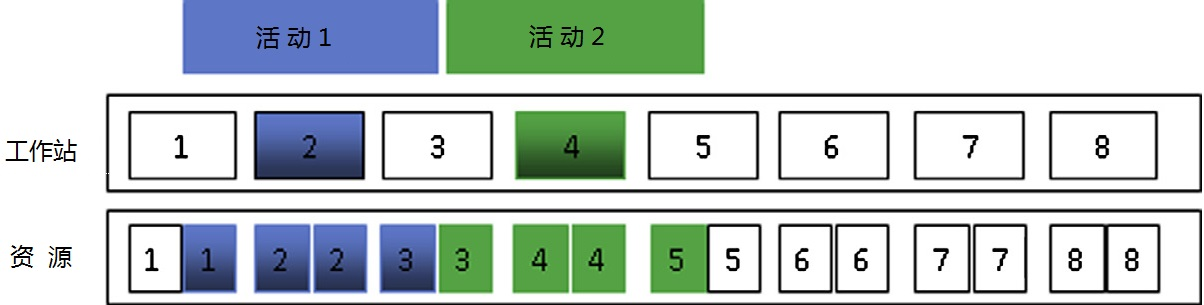
\includegraphics[width=12cm]{resourceandworkstation}
\end{figure}
\reff{fig:representationofresourcesandworkstations}举了一个例子,其中活动1在工作站2进行装配,它占用了2个工作站2的资源,其中1个是来自邻接工作站1,另一个来自邻接工作站3。
类似的,活动2占用2个工作站4的资源,其中1个来自邻接工作站3,另一个来自邻接工作站5。
因此,工作站1,3,5将被邻接约束所阻塞,不能和工作站2,4同时工作。
然而,任何使用工作站6,7,8的活动可以在处理活动1,2时同时进行。

进一步,整个调度周期可表示为多重时间周期$t = 1,...,T$,其中$T$表示每架飞机的生产周期。新增的参数模型如下:\\[3pt]
\indent $J:$ 活动数;

$T:$ 时间周期(时域)数;

$K:$ 夹具中的工作站数;

$W:$ 装配团队类型数;

$j:$ 活动,$j = 1,...,J$;

$t:$ 时间,$t = 1,...,T$;

$k:$ 资源类型,对应于各夹具的工作站,$k = 1,...,K$;

$w:$ 装配团队类型,$w = 1,...,W$;

$c_{jk}:$ 需要执行活动$j$的资源类型$k$的数量。注意$c_{jk} = 0$说明活动$j$没有在工作站$k$进行装配;

$C_k:$ 资源类型$k$的可用数量;

$p_j:$ 活动$j$的持续时间;

$n_{jw}:$ 需要执行活动$j$的类型$w$的工人数量;

$v_w:$ 装配队伍类型$w$的单位工人成本。

此外,对于每个活动对$(h,j)$,其中$h\neq j$,需要定义下面集合:
\begin{numcases}{}
H = \left\{(h,j)\mid\text{活动$h$先于活动$j$}\right\}\notag\\
G = \left\{(j)\mid\text{活动$j$在夹具上处理过,无论是哪个工作站}\right\}\notag
\end{numcases}

该模型的决策变量定义如下:
\begin{numcases}{x_{jt} = }
1 \qquad \text{如果活动$j$在时间$t$完成}\notag\\
0 \qquad \text{其他情况}\notag
\end{numcases}

$a_w:$ 类型$w$的资源需求量。特别的,由于模型用于求解阶段2,$W=2$,并且
\begin{center}
$a_1:$ 夹具内的工人需求量

$a_2:$ 工作台的工人需求量
\end{center}
如此一来,阶段2的数学模型如下:
\begin{align}
&\label{equb:11} \min \quad \sum_{w=1}^W v_wa_w\\
&\label{equb:12} \sum_{t=1}^T x_{jt} = 1,\qquad j = 1,...,J\\
&\label{equb:13} \sum_{t = r_h + p_h}^{d_h}t\cdot x_{ht}\leqslant \sum_{t = r_h + p_h}^{d_j}(t - p_j)x_{jt},\qquad \forall (h,j) \in H\\
&\label{equb:14} \sum_{j\in G}\sum_{b=t}^{\min\{t + p_j,T\}}c_{jk}x_{jb} \leqslant C_k,\qquad k = 1,...,K,\ t = 1,...,T\\
&\label{equb:15} \sum_{j=1}^J\sum_{b=t}^{\min\{t + p_j,T\}}n_{jw}x_{jb} \leqslant a_w,\qquad w = 1,...,W,\ t = 1,...,T\\
&\label{equb:16} x_{jt}\in \{0,1\},\ a_w\in Z^+,\ j = 1,...,J,\ t = 1,...,T,\ w = 1,...,W
\end{align}
在该模型中,目标函数(\ref{equb:11})最小化总人工成本,约束\eqref{equb:12}确保了每一个活动在水平时域中只调度过1次,约束\eqref{equb:13}确保各活动的先后关系,约束\eqref{equb:14}确保各资源的使用总和不超过其可利用值,\eqref{equb:15}确保各周期内的活动有充足的人工,\eqref{equb:16}参考决策变量的定义域。

注意每个周期$t$,约束\eqref{equb:14}和(\ref{equb:15})的左侧考虑了所有活动$j$在周期$t$前开始,并在$t$完成,即在区间$[t,t+p_j-1]$内完成,如\reff{fig:notinparallelt}所示。
\begin{figure}[h]
\centering\caption{在不平行的持续时间$t$内的活动\label{fig:notinparallelt}}
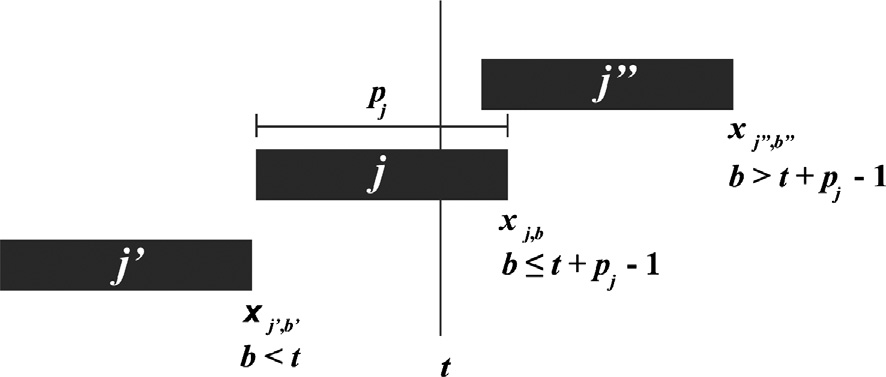
\includegraphics[width=8cm]{activitiesnotinparallel}
\end{figure}
如果在某个活动没有在周期$t$内处理,如$j'$和$j''$,那么它们不用在\eqref{equb:15}和(\ref{equb:15})的左边考虑。

需要考虑以下参数:\\[3pt]
\indent $EF_j:$ 活动$j$的最早可完成时间,表示在不考虑资源约束的先后关系;

$LF_j$活动$j$的最迟完成时间,不考虑项目延迟、先后关系和资源限制。

为防止某些活动的提交时间大于0,或者工期小于制造期(即防止与活动相关多架飞机,并且工期不同),我们需要定义:\\[3pt]
\indent $r_j:$ 活动$j$的可开始处理时间($r_j\geqslant EF_j - p_j$);

$d_j:$ 活动$j$的工期($d_j \leqslant LF_j$)。

所以上述模型可以简单地通过删除\eqref{equb:13}并增加下面的约束进行修改:
\begin{align}
&\label{equb:17}\sum_{t = \max\{EF_h,r_h + p_h\}}^{\min\{LF_h - 1,d_h - 1\}}t\cdot x_{ht}\leqslant \sum_{t =  \max\{EF_h,r_h + p_h\}}^{\min\{LF_h - 1,d_h - 1\}}(t - p_j)x_{jt} \qquad \forall (h,j)\in H\\
&\label{equb:18}x_{jt} = 0 \qquad t = 1,...,EF_j - 2,\ t = LF_j +1 ,...,T,\ j =1,..,J
\end{align}
其中,\eqref{equb:17}确保了所有活动的先后关系,约束\eqref{equb:18}确保了活动在其提交期和工期中被调度。这样可以在模型求解前消除已知值得变量,提高计算速度。

\eqref{equb:11} -- (\ref{equb:16})可以在离散时间内简单地改编成\eqref{equb:1} -- (\ref{equb:9})。由于在阶段1对劳动力没有限制,\eqref{equb:15}可以去除,目标函数(\ref{equb:11})可以写作:
\[ \centering\min\sum_{t=1}^T t\cdot x_{jt}
\]
其中$J$是先后关系网中的最后一个活动,然而,该模型并不完善,因为连续时间模型可以提供更短的计算运行时间。

\ksection{阶段3}
在阶段3,工人将分成两组,可在夹具内和工作台内操作的非专位组和只能在在工作台操作的专位组。此外,如阶段2模型所用到的参数,此处亦需考虑参数如下:\\[3pt]
\indent $s_{jw}:$ 需要在夹具内操作的活动$j$所需的$w$型资源数量;

$v_{jw}:$ 需要在工作台内操作的活动$j$所需的$w$型资源数量。

本文所研究的$j$操作问题只由单工人完成,因此$s_{jw}$和$v_{jw}$都等于1。阶段3的决策变量如下:
\begin{numcases}{x_{jt} = }
1 \qquad \text{如果活动$j$恰好在时间$t$完成}\notag\\
0 \qquad \text{其他情况}\notag
\end{numcases}\\[3pt]
\indent $a_w:$ 队伍$w$所需的工人数,在阶段3($W = 2$):

$a_1:$ 可以在工作台和夹具内操作的工人需求量;

$a_2:$ 只能在工作台操作而工人需求量。

需要注意的是,约束\eqref{equb:23}和(\ref{equb:24})引入了松弛变量$y_t$,表示在时间$t$可用于工作台的专位同人队伍冗余,阶段3的数学模型如下:
\begin{align}
&\label{equb:19} \min \qquad \sum_{w=1}^{W}v_wa_w\\
&\label{equb:20} \sum_{t = 1}^T x_{jt}  = 1,\quad j = 1,...,J\\
&\label{equb:21} \sum_{t = EF_h}^{LF_h -1}t\cdot x_{ht}\leqslant \sum_{t = EF_j}^{LF_j - 1}(t - p_j)x_{jt},\quad \forall (h,j) \in H\\
&\label{equb:22} \sum_{j\in G}\sum_{b=t}^{\min\{t + p_j-1,T\}}c_{jk}x_{jb}\leqslant C_k,\quad k = 1,...,K,\ t = 1,...,T\\
&\label{equb:23} \sum_{j\in G}\sum_{b=t}^{\min\{t + p_j-1,T\}}s_{jw}x_{jb} = a_w - y_t,\quad W = 1,\ t = 1,...,T\\
&\label{equb:24} \sum_{j\in J\backslash G}\sum_{b=t}^{\min\{t + p_j-1,T\}}v_{jw}x_{jb} = a_w + y_t,\quad W = 2,\ t = 1,...,T\\
&\label{equb:25} x_{jt} = 0,\qquad t = 1,...,EF_j - 2,\ t = LF_j +1 ,...,T,\ j =1,..,J\\
&\label{equb:26} x_{jt}\in \{0,1\},\ a_w \in Z^+,\ y_t \geqslant 0,\ t = 1,...,T,\ w = 1,...,W
\end{align}
目标函数(\ref{equb:19})最小化可用工人的总成本,\eqref{equb:20}保证了所有活动只被调度一次,\eqref{equb:21}保证了所有活动遵循其先后关系,\eqref{equb:23}确保了夹具内工人数量足够,\eqref{equb:24}确保了工作台内工人数量足够,\eqref{equb:25}修正了已知变量,\eqref{equb:26}参考变量的定义域。
注意在约束\eqref{equb:23}和(\ref{equb:24})中,$x_{jb},a_w,s_{jw},v_{jw}$为整数,保证了$y_t$的完整性。因此,\eqref{equb:26}中强调$y_t$是非负实数是必要的。

\ksection{阶段4}
在阶段4,装配组的所有工人可以在夹具和工作台内操作。由于工人间没有技能区别,为阶段2建立的数学模型可以用于这个阶段,在\eqref{equb:11} -- (\ref{equb:16})只要考虑一类工人($W = 1$)即可。这个阶段是学习曲线的最后阶段,所有工作都是多任务的。
在这个阶段,需要考虑较小增长的生产率,有着较大的影响。最优化队伍规模要比前阶段更为重要,因为这个阶段大部分飞机已完工。
% !Mode:: "TeX:UTF-8"
% !TEX root = ..\Literature_Translation.tex
\kchapter{计算结果}
使用建模语言GAMS(v23.0)建立该数学模型,并用CPLEX 11.2.1.0 使用4核求解。计算实验在一台处理器为Intel i7(2.8GHz, 12GB)的PC 机上运行,所有示例实验时间设为10 h。

这些示例包括15个活动,通常这些活动在工作台上的操作时间要长于夹具。
为了保护公司数据的隐私性,持续时间的单位(t.u.)不表示实际时间,因为其乘上了一个常数。需要注意的是,每架飞机需要两整套装配子集,因此,活动数目被扩大成30个活动。

\begin{table}[htbp]
  \centering
  \caption{Add caption}
    \begin{tabular}{ccccccc}
    \toprule

子集 &子集的零件 &活动(j) &\multicolumn{1}{m{20mm}}{夹具中的工作站} &\multicolumn{1}{m{20mm}}{夹具中的持续时间(mj)} &  \multicolumn{1}{m{20mm}}{工作台上的持续时间(qj)} &  \multicolumn{1}{m{20mm}}{前继活动(A(j,k)) }\\
\midrule
    1     & 1     & 1     & 1     & 5     & 7     & - \\
    1     & 1     & 2     & 1     & 4     & 47    & 1 \\
    2     & 1     & 3     & 1     & 5     & 7     & - \\
    2     & 1     & 4     & 1     & 4     & 47    & 3 \\
    1     & 2     & 5     & 2     & 15    & 29    & - \\
    1     & 2     & 6     & 2     & 9     & 71    & 5 \\
    2     & 2     & 7     & 2     & 15    & 29    & - \\
    2     & 2     & 8     & 2     & 9     & 71    & 7 \\
    1     & 3     & 9     & 3     & 11    & 40    & - \\
    2     & 3     & 10    & 3     & 11    & 40    & - \\
    1     & 4     & 11    & 4     & 12    & 40    & - \\
    1     & 4     & 12    & 4     & 6     & 40    & 11 \\
    2     & 4     & 13    & 4     & 12    & 40    & - \\
    2     & 4     & 14    & 4     & 6     & 40    & 13 \\
    1     & 5     & 15    & 5     & 8     & 30    & - \\
    1     & 5     & 16    & 5     & 6     & 40    & 15 \\
    2     & 5     & 17    & 5     & 8     & 30    & - \\
    2     & 5     & 18    & 5     & 6     & 40    & 17 \\
    1     & 6     & 19    & 6     & 12    & 17    & - \\
    1     & 6     & 20    & 6     & 6     & 40    & 19 \\
    2     & 6     & 21    & 6     & 12    & 17    & - \\
    2     & 6     & 22    & 6     & 6     & 40    & 21 \\
    1     & 7     & 23    & 7     & 7     & 12    & - \\
    1     & 7     & 24    & 7     & 7     & 30    & 23 \\
    2     & 7     & 25    & 7     & 7     & 12    & - \\
    2     & 7     & 26    & 7     & 7     & 30    & 25 \\
    1     & 8     & 27    & 8     & 10    & 61    & - \\
    1     & 8     & 28    & 8     & 12    & 66    & 27 \\
    2     & 8     & 29    & 8     & 10    & 61    & - \\
    2     & 8     & 30    & 8     & 12    & 66    & 29 \\
    \bottomrule
    \end{tabular}%
  \label{tab:addlabel}%
\end{table}%
